\documentclass[]{article}
\usepackage[koi8-r]{inputenc}
\usepackage{geometry}
\usepackage[pdftex]{graphicx}
\usepackage{wrapfig}
\graphicspath{{../images/}}
\DeclareGraphicsExtensions{.png}
%opening
\title{Astrometric Observations of the Main Uranian Satellites in the Pulkovo Observatory in 2007 -- 2016}
\author{Ershova A. P., Roschina E. A., Izmailov I. S., Khovrichev M. Yu.}
\geometry{left=2.5cm}
\geometry{right=2.5cm}
\geometry{top=2cm}
\geometry{bottom=2cm}
\begin{document}

\maketitle

\begin{abstract}

\end{abstract}

\section{Introduction}
High-precision theories of motion of the major planets and their satellites  are necessary for reserches of formation and evolution of the Solar System and for providing the ephemerides to the future space missions. Elaboration of such theories requires an extensive observational material. N.V. Emel'anov in his article \cite{4} pointed that precision of ephemerides can be improved via extansion of the observational span.\par

In the twentieth century photographic observations of Uranus were performed in the Pulkovo Observatory \cite{8}. Coordinates of the planet were mesaured directly, uranian satellites were inaccessible for the photographic method.\par

Observations of Uranus with the CCD-camera have started in 2007. In CCD frames it is possible to receive siutable for mesaurements images of four main uranian satellites: Ariel (u1), Umbriel (u2), Titania (u3) and Oberon (u4). Precision of mesaurements for these satellites appears so good as in other works on the same subject.\cite{2, 7}. The fifth main satellite of Uranus is Miranda (u5), which is at small angular distant from the planet. Therefore its images in frames are cannot be separated from Uranus halo.\par

The first results of observations of uranian satellites with CCD-camera and 26-inch refractor in Pulkovo were published in 2013 in article of Roschina et al. \cite{1}. Published observations covered 2007 -- 2011 period. UCAC2 was used as a reference catalogue. Volume of observational data in current paper is much bigger: observations cover period since August 2007 to Janiary 2016. The mesaurements were performed with UCAC4 \cite{9}, thus there were more stars in the field of view.

\section{Observations and mesaurements}
Current observations of Uranus are performing in Pulkovo from the end of August to the begining of Janiary. The used telescope is the 26-inch refractor, which is located on $59^o46' 15''$ north latitude, $30^o19'23''$ east longitude, altitude above sea level is about 85 m.  Aperture diameter of the teleskope is 65 cm, focal length is 1041.3 cm, focal plane scale is $19''.80$/mm in the center of image. The CCD camera FLI Pro Line 09000  is used as a radiation receiver. Size of the CCD matrix is $3056$x$3056$ px, each of 12 $\mu$m.  The field of view is $12'$x$12'$, the scale on the CCD frames is $0''.24$/px.\par
One normal place of each satellite available for observations was calculated on a basis of five independent mesaurements of individual positions.  In turn for each of these mesaurements a number of CCD frames combined together was used. Observations were carried out by series: September 30, 2007 -- 20 frames with expositions of 20 s (were sumed on 4), October, 21, 2007 -- 130 frames with exposition of 3 s (were sumed on 25), on 40 frames with expositions of 10 seconds (sumed on 8) in all other nights. Movement of satellites on the celestrial sphere during observation was approximated linearly, the average moment for all series and the normal place corresponding to this moment was calculated.\par
Observations processing and coordinate mesaurements were performed with the IZMCCD software package developed by I.S. Izmailov \cite{3,4}. In case when an image of satellite was contaminated by planet halo the halo was subtracted by approcsimation of brightness distribution with series of negative degrees on a formula (\ref{2}). Coefficients $a, b, c, d$ is estimated by the least square method. $r$ is the distance to a certain point which coordinates are also selected via minimization of discrepancies.\par
\begin{equation}
\label{2}
I(r) = a + \frac{b}{r} + \frac{c}{r^2} + \frac{d}{r^3}
\end{equation}
Image center coordinates of satellites and reference stars in the frame plane was calculated using the Lorenz function approximation (\ref{1}).


\begin{equation}
\label{1}
I(x,y) = \frac{C}{(1 + AR)^{\alpha}} + D
\end{equation}
\begin{center}
\begin{math}
R = \sqrt{(x-x_0)^2 + (1+B)(y-y_0)^2 +E(x-x_0)(y-y_0)}
\end{math}\\
\end{center}
$I(x,y)$ -- brightness in the pixel which coordinates are ($x$, $y$)\par
$(x_0, y_0)$ -- coordinates of image center\par
$\alpha$ --  determine the form of the curve, in our case $\alpha = 1.4$\par
$A$, $B$, $C$, $D$, $E$ -- parameters of model:\par
$A$ -- sets the size of image\par
$B$ -- elongation of the image on an axis $y$\par
$C$ -- brightness in the center of image\par
$D$ -- constant term\par
$E$ -- elongation of the image on arbitrary direction\par
\vskip0.1cm

The Lorenz function parameters were obtained  solving excess system of equations by the non-linear method of the least squares. Then coordinates of centers of satellites and stars images in the plane of CCD image were calculated. Astrometric reduction was performed by the six-constant method. During reduction the differential refraction of the first order was considered. UCAC4 \cite{9} was taken as a reference catalog. In the field of view at least 8 stars from UCAC4 were founded. The majority of pictures were identified more than on 10 stars. \par
Errors of measurements were estimated on standard formulas.

\begin{math}
\sigma_x = \sqrt{\frac{\sum\limits_{k=1}^{N}(x_k-x_{mean})^2}{N-1}}; \varepsilon_x = \sigma_x/\sqrt{N}
\end{math}\\

If error of mesaurement of the individual position was greater then $0.''3$ for Ariel and Umbriel or greater $0.''1$ for Titania and Oberon, such mesaurement of that night of that satellite was thrown out from further consideration. Average values of errors passed the specified criterion are shown in the table \ref{errors}.\par
\begin{table}[h!]
\caption{Average errors of normal places $\varepsilon$ and average errors of individual position $\sigma$ (arcsec)}
\label{errors}
\begin{center}
\begin{tabular}{|c|c|c|c|c|}
\hline
&Ariel&Umbriel&Titania&Oberon \\
\hline
$\varepsilon_\alpha (\sigma_\alpha)$&0.06 (0.11)&0.05 (0.09)&0.02 (0.03)&0.02 (0.03) \\
$\varepsilon_\delta (\sigma_\delta)$&0.06 (0.11)&0.07 (0.11)&0.02 (0.03)&0.02 (0.04) \\
\hline
\end{tabular}
\end{center}
\end{table}



\section{Results and comparing with theory}
Almost 7000 CCD images of Uranus and its satellites were collected from 2007 to 2016. In the table \ref{number_of_points} it is shown how many nights each of four satellites was observed, that corresponds to number of the normal places received during a year, there is the quantity of the individual positions measured for all year in brackets.\par

\begin{table}
\caption{The quantity of the normal places and the individual positions measured for a year}
\label{number_of_points}
\begin{center}
\begin{tabular}{|c|c|c|c|c|c|c|c|c|c|}
\hline
 & 2007 & 2008 & 2009 & 2010 & 2011 & 2012 & 2013 & 2014 & 2015\\
\hline
Ariel & 0(0) & 0(0) & 3(15) & 0 (0) & 0(0) & 2 (10) & 2 (10) & 2 (10) & 7 (35)\\
Umbriel & 0(0) & 2 (10) & 4 (20) & 4 (20) & 4 (20) & 4 (20) & 14 (70) & 8 (40) & 11(55)\\
Titania & 3 (13) & 5 (25) & 11 (55) & 5 (25) & 15 (75) & 12 (60) & 19 (91) & 15 (74) & 21 (105)\\
Oberon & 4 (21) & 7 (35) & 11 (55) & 5 (25) & 18 (90) & 13 (65) & 18 (88) & 19 (94) & 21 (105) \\
\hline
\end{tabular}
\end{center}
\end{table}
Obtained normal places are not distributed on the whole period evenly. There is tendency toward increasing of number of obtained positions from 2007 to 2016. This effect was noticed in the paper of Camargo et. al. \cite{2} It is explained by changing of the angle between the equatorial plane of Uranus and the picture plane. In the begining of observational span the equatorial plane of the planet, also the orbital planes of satellites, were almost perpendicular to the plane tangential to the celestial sphere. Thereof, the uranian satellites spent most time behind the planet or right in front of it, so their coordinates could not be mesaured on CCD frame. In process of the movement on an orbit around the Sun Uranus is turning around so, that the angle between its equatorial plane and plane of an image is decreasing.
\begin{wrapfigure}[12]{r}{0.4\linewidth} 
\vspace{-4ex}
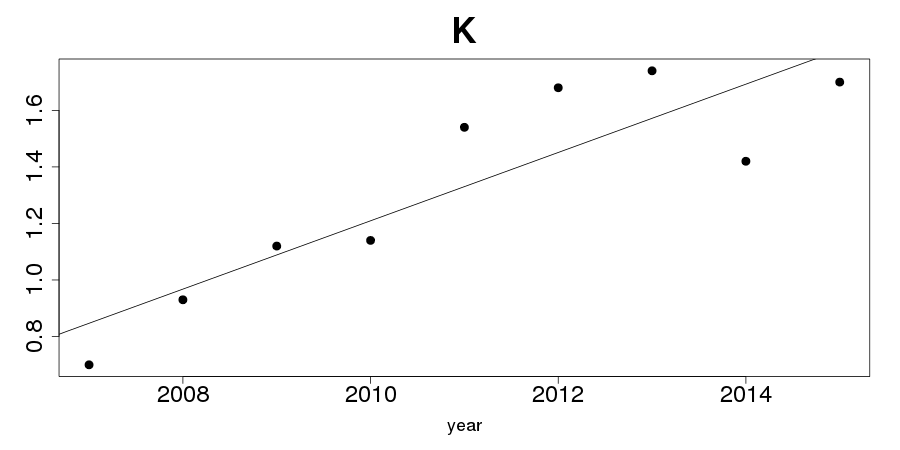
\includegraphics[width=\linewidth]{K}
\caption{The ratio of the normal places obtained during a season to the number of observational nights}
\label{fig:K}
\end{wrapfigure}

 Thus the satellites appear in the CCD frame at sufficient distance from the planet that their coordinates could be mesaured.\par
Let's show this effect colculating the $K$ coefficient that is the ratio of the normal places obtained during an observational season to the number of nights in this season when a series of frames with Uranus was made. The observation season is meant as the period since the end of August on the beginning of January, January observation nights are attributed to previous year. Figure (\ref{fig:K}) illustrates the increase in this ratio.\par


Obtained coordinates were compared with coordinates predicted with the planet motion theory the INPOP13c and the theory of uranian satellite motion Lainey 2015. The ephemerides were provided by the MULTI-SAT servise\cite{5}. Also positions of Uranus were determined based on the positions of its satellites and ephemeris distanses between them and the planet.  The series of the O-C differences for each satellite and for the planet are shown on the plots, the average O-C differences are in the table \ref{mean_OC}.

\begin{table}
\begin{center}
\caption{The average O-C differences}
\label{mean_OC}
\begin{tabular}{|c|c|c|c|c|c|}
\hline
& Ariel&Umbriel&Titania& Oberon & Uranus \\
\hline
Average $(O-C)_\alpha$ & 0.043 & 0.025 & -0.009 & -0.001 & 0.001\\
Average $(O-C)_\delta$ & -0.074 & -0.069 & -0.014 & -0.019 & -0.021\\
\hline
\end{tabular}
\end{center}
\end{table}

\begin{figure}[h!]
\begin{minipage}[h]{0.49\linewidth}
\centering{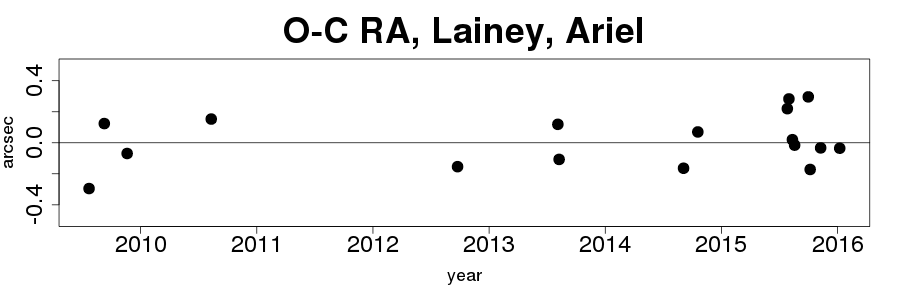
\includegraphics[width=1.0\linewidth]{Ariel_Lainey_RA}\\Ariel, $(O-C)_\alpha$}
\end{minipage}
\begin{minipage}[h]{0.49\linewidth}
\centering{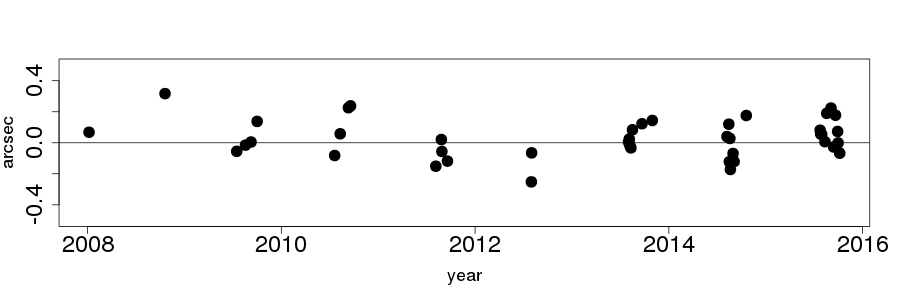
\includegraphics[width=1.0\linewidth]{Umbriel_Lainey_RA}\\Umbriel, $(O-C)_\alpha$}
\end{minipage}
\end{figure}
\begin{figure}[h!]
\begin{minipage}[h]{0.49\linewidth}
\centering{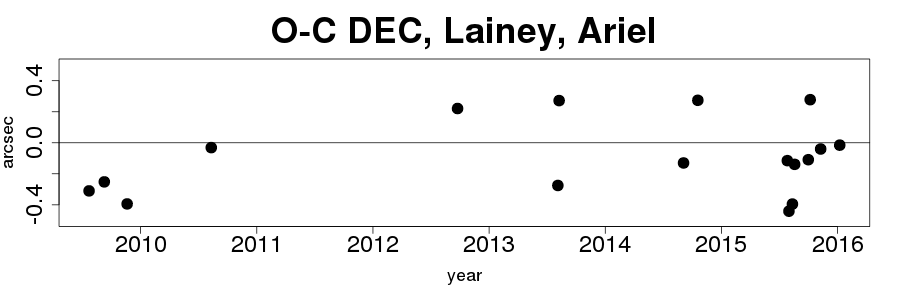
\includegraphics[width=1.0\linewidth]{Ariel_Lainey_DEC}\\Ariel, $(O-C)_\delta$}
\end{minipage}
\begin{minipage}[h]{0.49\linewidth}
\centering{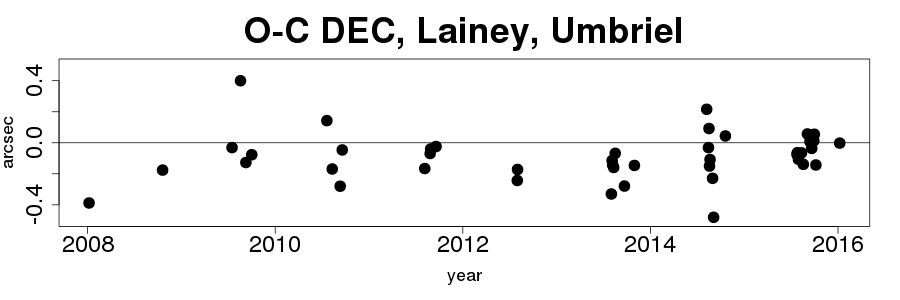
\includegraphics[width=1.0\linewidth]{Umbriel_Lainey_DEC}\\Umbriel, $(O-C)_\delta$}
\end{minipage}
\end{figure}


\begin{figure}[h!]
\begin{minipage}[h]{0.49\linewidth}
\centering{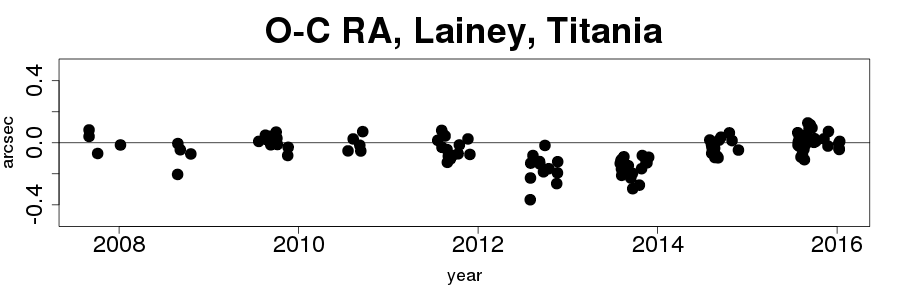
\includegraphics[width=1.0\linewidth]{Titania_Lainey_RA}\\Titania, $(O-C)_\alpha$}
\end{minipage}
\begin{minipage}[h]{0.49\linewidth}
\centering{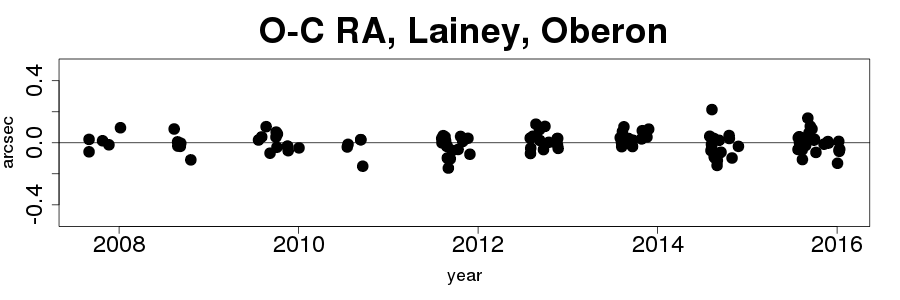
\includegraphics[width=1.0\linewidth]{Oberon_Lainey_RA}\\Oberon, $(O-C)_\alpha$}
\end{minipage}
\end{figure}
\begin{figure}[h!]
\begin{minipage}[h]{0.49\linewidth}
\centering{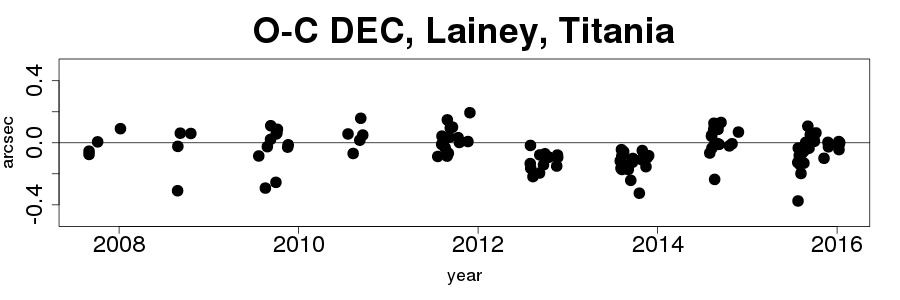
\includegraphics[width=1.0\linewidth]{Titania_Lainey_DEC}\\Titania, $(O-C)_\delta$}
\end{minipage}
\begin{minipage}[h]{0.49\linewidth}
\centering{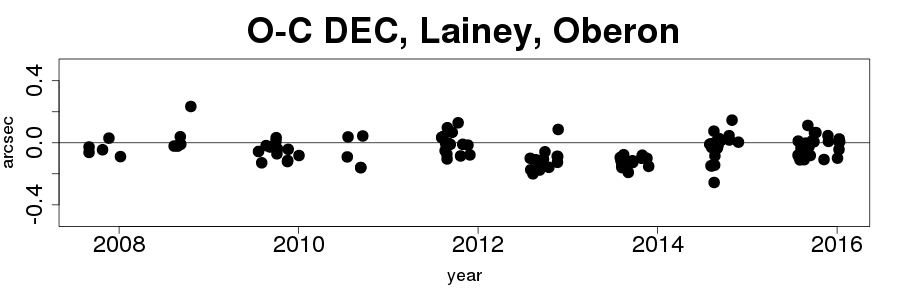
\includegraphics[width=1.0\linewidth]{Oberon_Lainey_DEC}\\Oberon, $(O-C)_\delta$}
\end{minipage}
\end{figure}


\begin{figure}[h!]
\begin{minipage}[h]{0.49\linewidth}
\centering{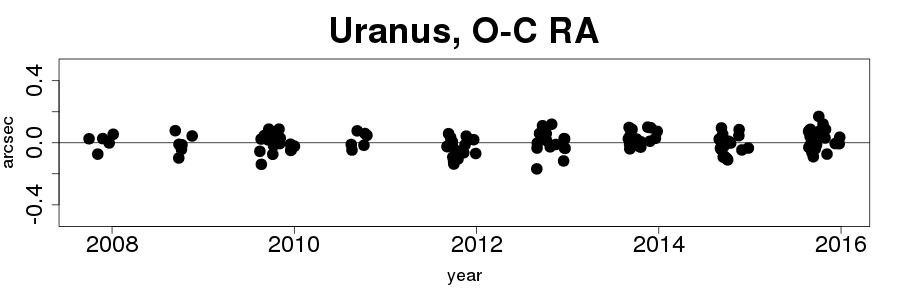
\includegraphics[width=1.0\linewidth]{Uranus_oc_ra}\\Titania, $(O-C)_\alpha$}
\end{minipage}
\begin{minipage}[h]{0.49\linewidth}
\centering{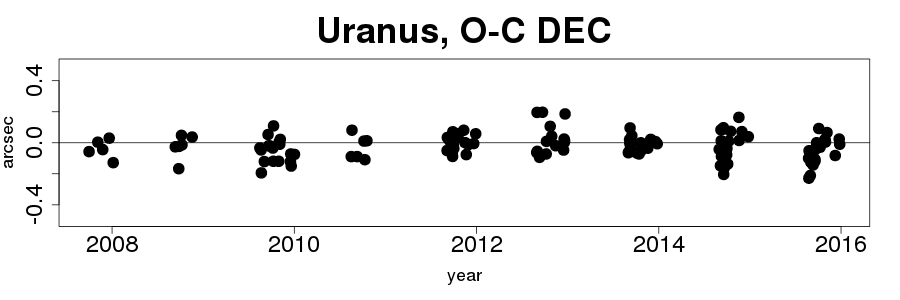
\includegraphics[width=1.0\linewidth]{Uranus_oc_de}\\Oberon, $(O-C)_\alpha$}
\end{minipage}
\end{figure}

 Observations show a good consent with theory.\par

\section{Conclusion}
This article reports the results of observations of the uranian satellites performed in Pulkovo Observatory with the 26-inch refractor in 2007 -- 2016. Analysis of the results demonstrates their high-quality and the suitability of the methods realised in this work, in particular, the method of planet halo subtracting. These methods can be applied in the future works on close subjects. Observed positions of the main uranian satellites are usually close to ephemeris position. The obtained normal places are avaliable in the pulkovo database and in the CDS database.

\section{Acknowledgments}





\begin{thebibliography}{99}
\bibitem{1} \textquotedblleft Astrometric Observations of Satellites of Uranus Using 26-Inch Refractor in 2007--2011\textquotedblright, 2013, E. A. Roschina, I. S. Izmailov, T. P. Kiseleva
\bibitem{2}  \textquotedblleft Astrometry of the main satellites of Uranus: 18 years of observations\textquotedblright, 2015, J.I.B. Camargo, F. P. Magalhaes, R. Vieira-Martins, M. Assafin, F. Braga-Ribas, A. Dias-Oliveira,G. Benedetti-Rossi, A. R. Gomes-Junior, A. H. Andrei and D. N. da Silva Neto
\bibitem{7} M.Yu. Khovrichev, Astrometric observations of the Uranian satellites with the Faulkes telescope North in 2007 September, 2009
\bibitem{6} Izmailov I.S., Kiselev A.A., Kiseleva T.P., and Khrutskaya E.V., Using a CCD-camera in Pulkovo programs of observations of binary and multiple stars and satellites of major planets with the 26-inch refractor . Astron. Lett., 1998, vol. 24, no. 5, pp. 665-672.
\bibitem{3}  Izmccd is a software  packet for processing digital images of celestial objects, 2005, Izmailov, I.S., http://www.izmccd.puldb.ru/
\bibitem{4} \textquotedblleft Precision of the ephemerides of outer planetary satellites\textquotedblright, Planetary and Space Science, 2009, Emelyanov N.V.
\bibitem{5} Emel'anov N/V/ and Arlot J.-E., The natural satellites ephemerides facility MULTI-SAT, Astron., Astrophis., 2008, vol. 487, pp. 759-765
\bibitem{8} Kiseleva T.P., Khrutskaya E.V., Pulkovo astrometric observations of bodies of the Solar System from 1898 to 2005: observational database, Solar. Syst. Res., 2007 vol. 41, no. 1, pp. 72-80
\bibitem{9} Zacharias, N.; Finch, C. T.; Girard, T. M.; Henden, A.; Bartlett, J. L.; Monet, D. G.; Zacharias, M. I., The Fourth US Naval Observatory CCD Astrograph Catalog (UCAC4), The Astronomical Journal, Volume 145, Issue 2, article id. 44, 14 pp. (2013)
\end{thebibliography}






\end{document}
